\documentclass{article}
\usepackage{amsmath}
\usepackage{amssymb}
\newcommand*{\qed}{\hfill\ensuremath{\blacksquare}}
\usepackage{graphicx}
\graphicspath{{.}}

\title{Computational Linear Algebra, Module 8}
\author{Maya Shende}
\date{Due: April 11th, 2018}

\begin{document}
\maketitle

\begin{enumerate}

%exercise 1
\item "fundamental theorem of a" yields the following completions:
\begin{enumerate}
	\item fundamental theorem of algebra
	\item fundamental theorem of arithmetic
\end{enumerate}
"fundamental theorem of b" yields the following completions:
\begin{enumerate}
	\item fundamental theorem of boolean algebra
	\item fundamental theorem of biomedical informatics
\end{enumerate}
"fundamental theorem of j" is the first search term that seems to fail.

%exercise 2
\item 
\begin{eqnarray*}
	x_1 &=& -x_3 - x_4 - 2x_5\\
	x_2 &=& -x_3 + x_4 + x_5
\end{eqnarray*}\\
When $x_3 = 1, x_4 = 0, x_5 = 0$, $x_1 = -1$ and $x_2 = -1$. \\
When $x_3 = 0, x_4 = 0, x_5 = 1$, $x_1 = -2$ and $x_2 = 1$. 

%exercise 3
\item drawing:\\
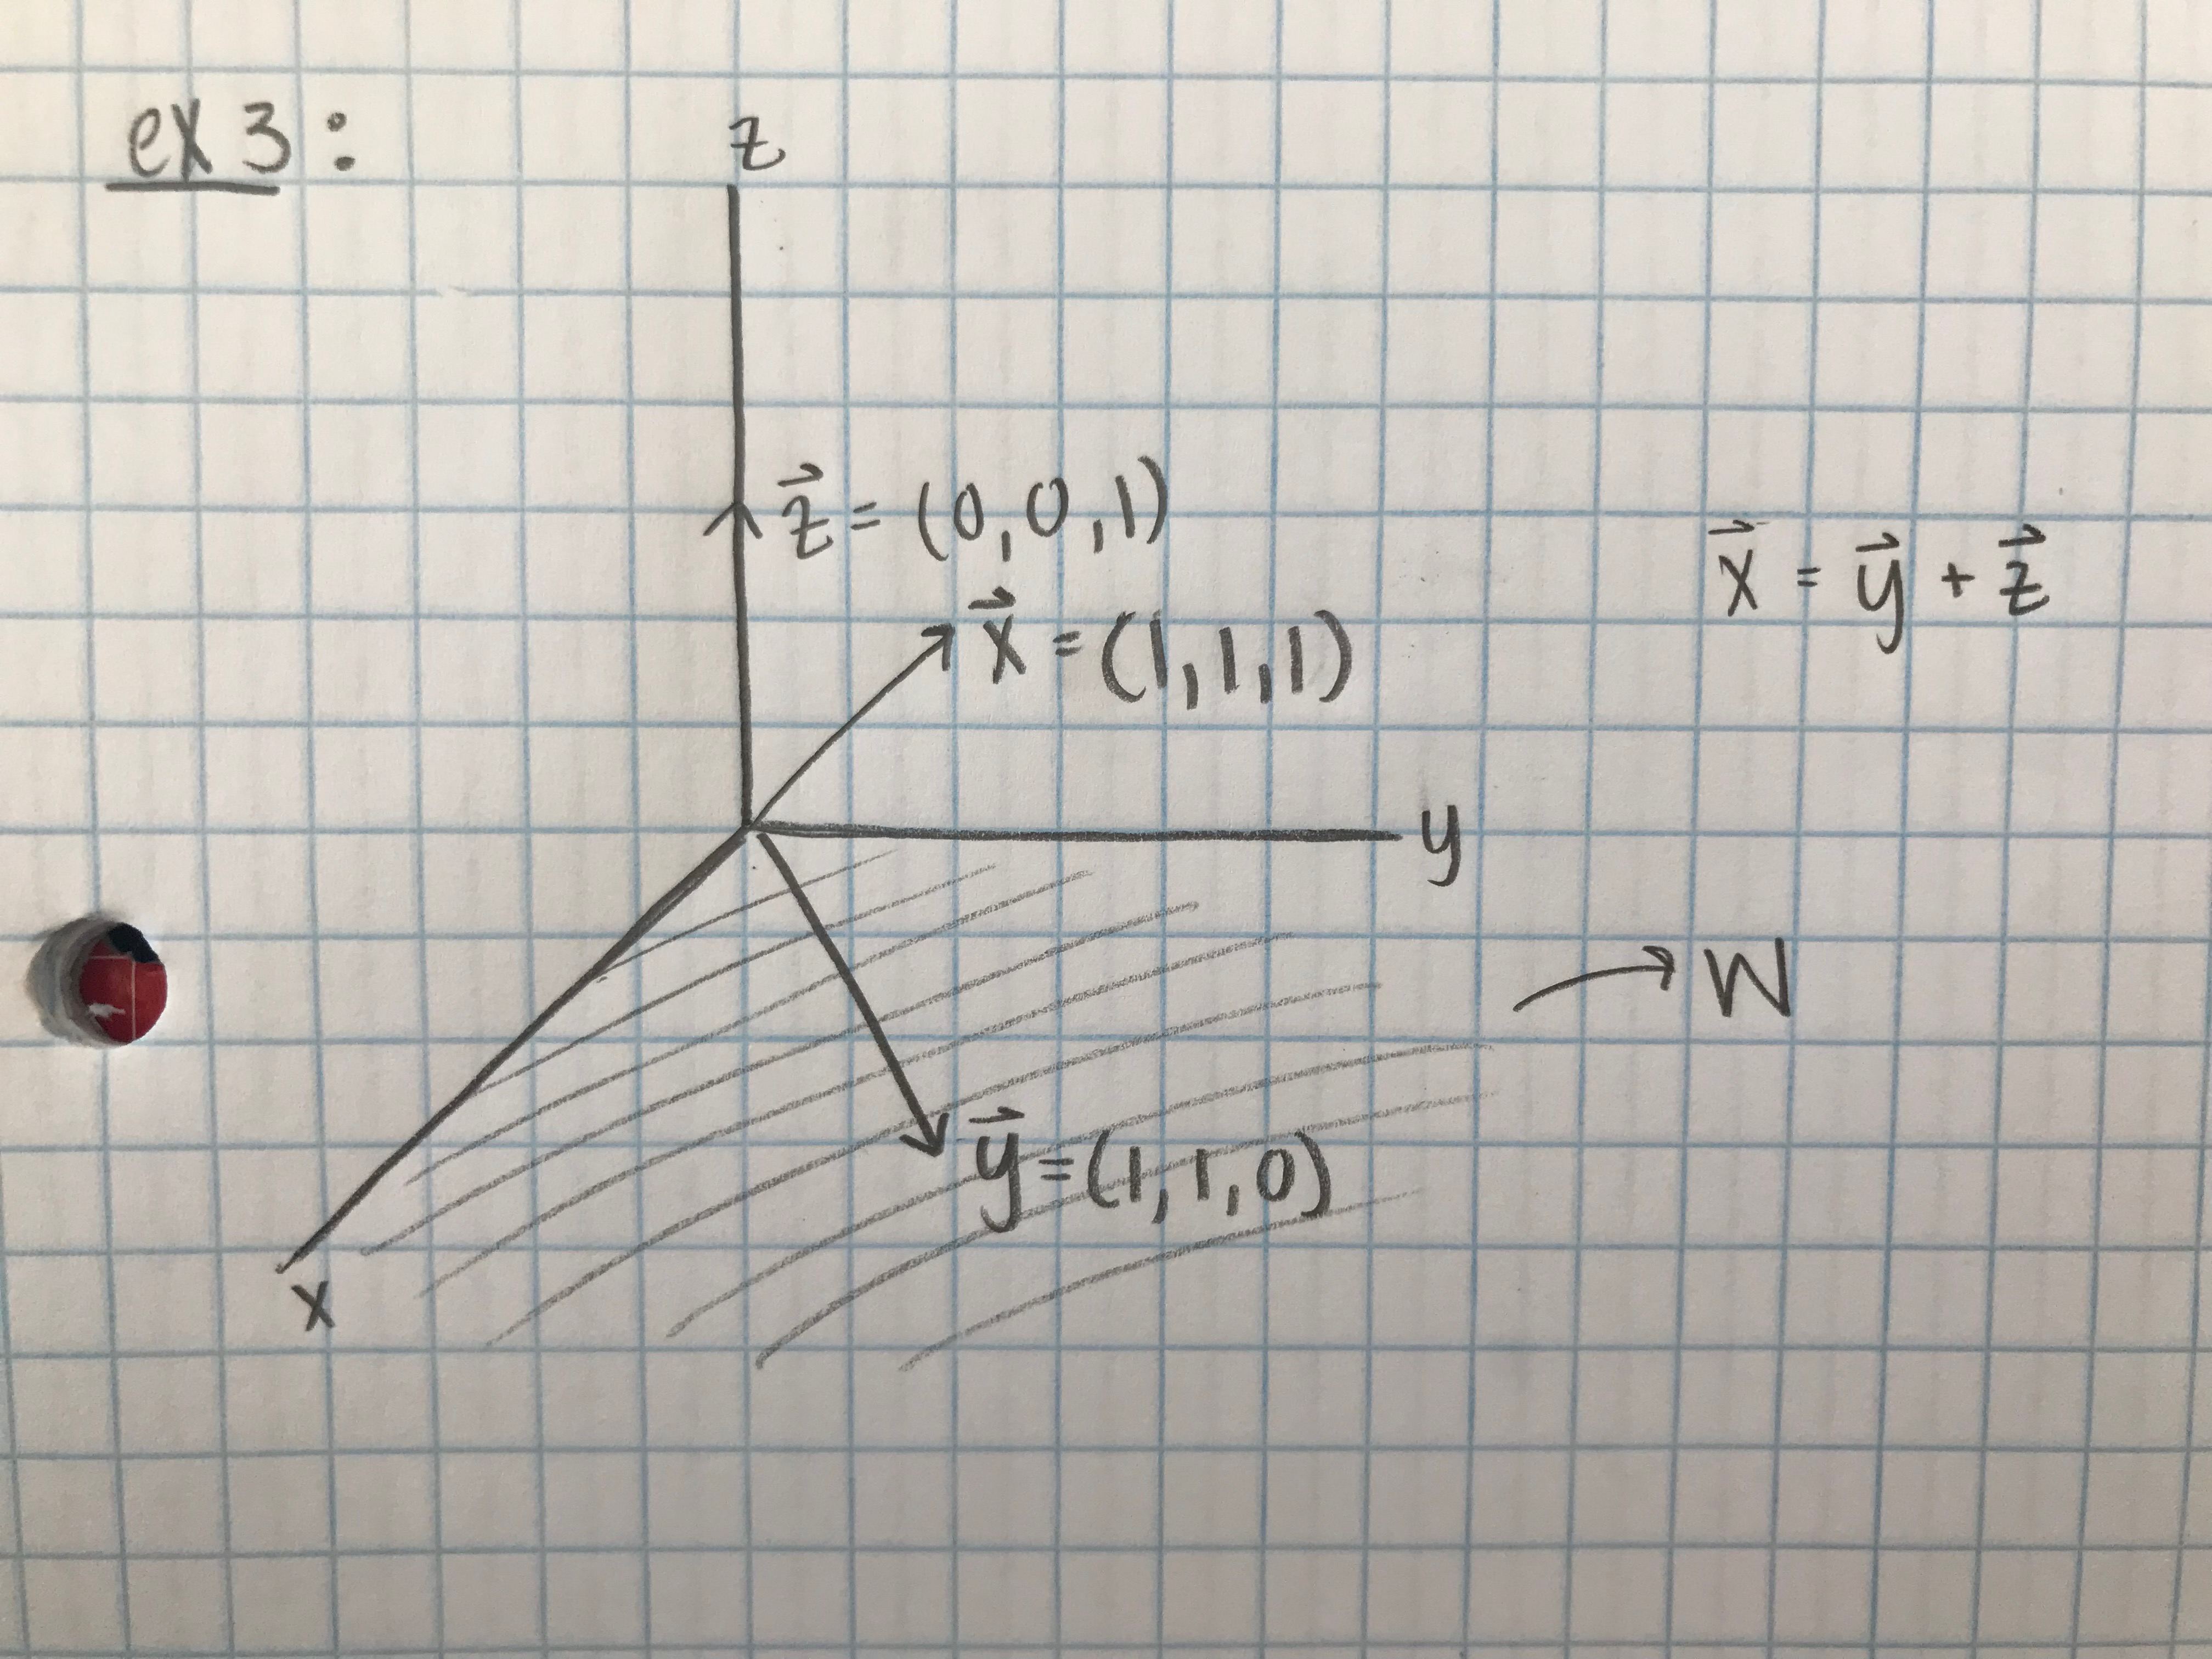
\includegraphics[scale=0.05]{exercise3}

%exercise 4
\item We know that the dim(W) = r, and we also know that the dimension of n-D space is n. So, if $W^{\perp}$ is the set of all vectors orthogonal to W, then it must have dimension $n-r$. 

%exercise 5
\item The nullspace of A is the set of all vectors that are orthogonal to A. Since z is the nullspace(A), $Az=0$ by definition. 

%exercise 6
\item By multiplying A and the rowspace of A, you will only get the columns of A that have a pivot in them, therefore b is the columnspace of A. 

%exercise 7
\item Suppose A is an $m \times n$ matrix with rank r. By Theorem 8.3, we know dim(nullspace($A$)) = n-r. We also know that $A^TA$ is an $n \times n$ matrix. By proposition 8.5, nullspace(A) = nullspace($A^TA$)), and by Theorem 8.3, dim(nullspace($A$))=dim(nullspace($A^TA$))=n-r. Now, since both $A$ and $A^TA$ have $n$ columns, we can conclude that $A^TA$ also has rank r. Thus, rank($A$) = rank($A^TA$). \qed

%exercise 8
\item $k=1$:\\
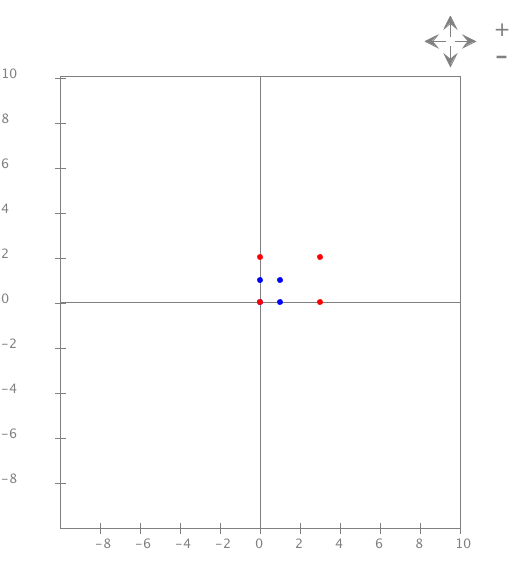
\includegraphics[scale=0.4]{exercise8_k1}\\
\item $k=3$:\\
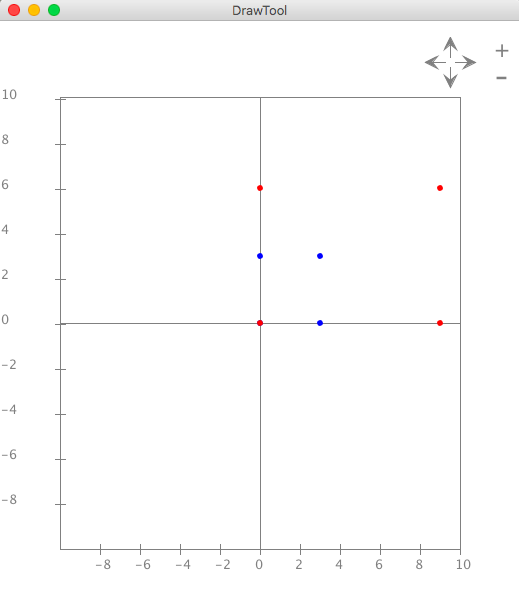
\includegraphics[scale=0.4]{exercise8_k3}\\
\item $k=5$:\\
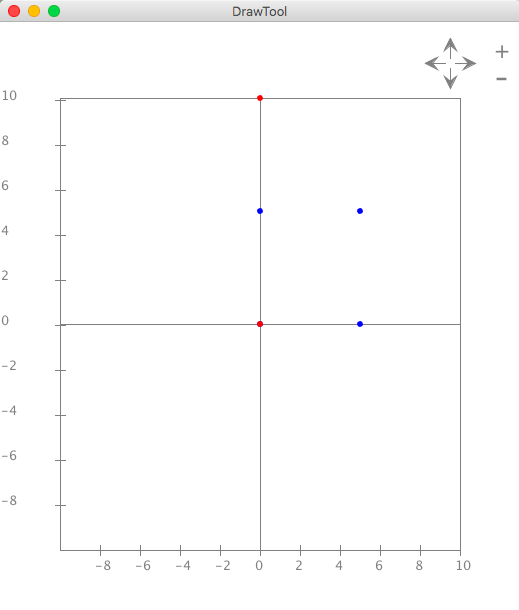
\includegraphics[scale=0.4]{exercise8_k5}\\

%exercise 9
\item need to do still

%exercise 10
\item $A=B$\\
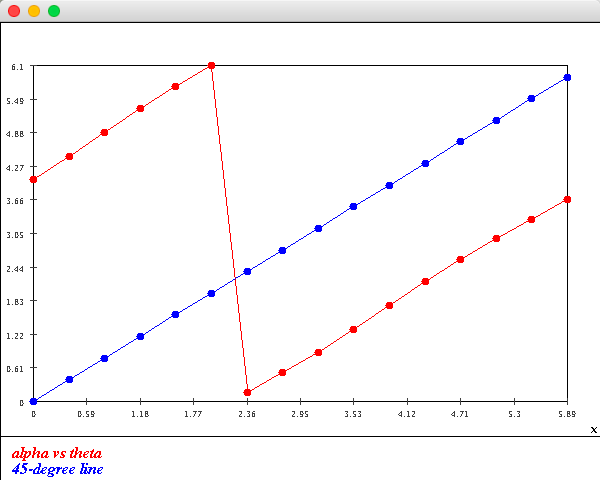
\includegraphics[scale=0.3]{exercise10_original}\\
$A=U$\\
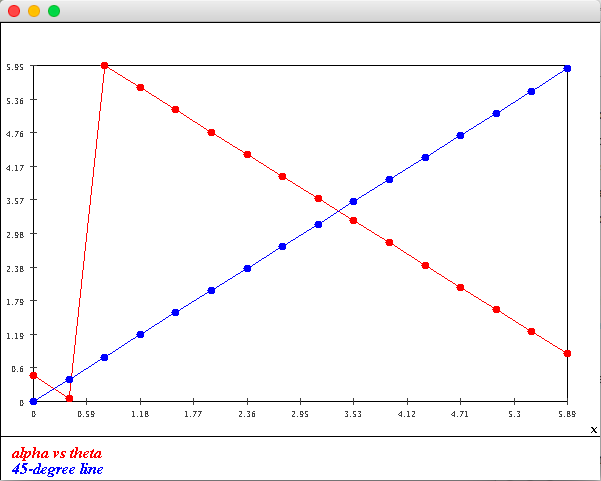
\includegraphics[scale=0.3]{exercise10_u}\\
$A=V$\\
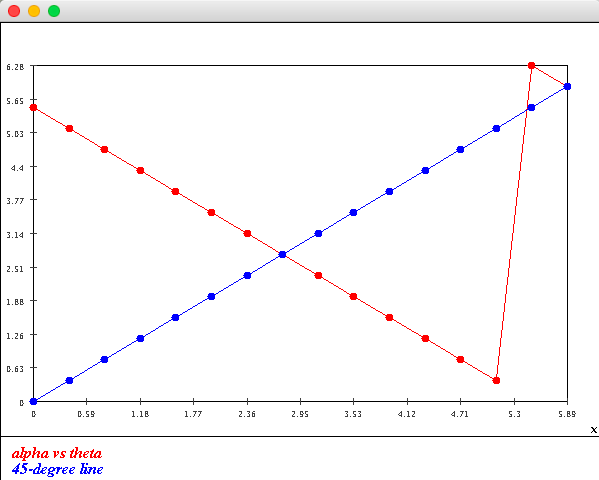
\includegraphics[scale=0.3]{exercise10_v}

%exercise11
\item 

%exercise 12
\item the dimensions of x and y are the dimensions of the matrix A, where the dimension of x is the number of columns in A and the dimension of y is the number of rows in A. 

%exercise 13
\item

%exercise 14
\item 

%exercise 15
\item 

%exercise 16
\item the standard vectors for $n=4$ are $(1, 0, 0, 0)$, $(0, 1, 0, 0)$, $(0, 0, 1, 0)$, and $(0, 0, 0, 1)$. 

%exercise 17
\item 

%exercise 18
\item 

%exercise 19
\item The transformation is linear which is why we can pull terms out like this.
\end{enumerate}
\end{document}